% Edit only the text between matching begin and end lines.
\documentclass[11pt,a4paper]{article}
% Shared preamble for TMUA question papers. Local edits here are overwritten.

% Reproducible PDFs: no timestamps, no trailer id, no build-path details.
\ifdefined\pdfsuppressptexinfo
  \pdfsuppressptexinfo=-1
  \pdfinfoomitdate=1
  \pdftrailerid{}
\fi

\usepackage{graphicx}
\usepackage{mathtools}
\usepackage{amssymb}
\usepackage{amsmath}
\usepackage{amsthm}
\usepackage{enumitem}
\usepackage{microtype}
\usepackage[table]{xcolor}
\usepackage{array}
\usepackage{booktabs}
\usepackage{tabularx}
\usepackage{longtable}
\usepackage{ragged2e}
\usepackage{fancyhdr}
\usepackage{etoolbox}
\usepackage[
  a4paper,
  left=0.8in,
  right=1in,
  top=1in,
  bottom=0.5in,
  headheight=14pt,
  headsep=0.4in
]{geometry}

\usepackage{pgfplots}
\pgfplotsset{compat=1.18}
\usepgfplotslibrary{fillbetween, polar}
\usetikzlibrary{calc, positioning}
\usetikzlibrary{angles, quotes}
\usetikzlibrary{arrows.meta}
\usetikzlibrary{decorations.pathreplacing, decorations.markings}
\usetikzlibrary{patterns}
\usetikzlibrary{intersections}

\usepackage{tocloft}
\usepackage[hidelinks]{hyperref}
\hypersetup{pdfauthor={danieljsmith.org}, pdfcreator={}, pdfsubject={}, pdfkeywords={}}
\urlstyle{same}
\tocloftpagestyle{djspaper}
\setlength{\cftbeforesubsecskip}{2pt}
\setlength{\cftsubsecindent}{1.5em}
\setlength{\cftsubsecnumwidth}{0pt}
\renewcommand{\cftsubsecfont}{\small\color{black}}
\renewcommand{\cftsubsecpagefont}{\small\color{black}}
\renewcommand{\cftsubsecleader}{\hfill}

% \djsPaperSetup{<PDF title>}{<header label>}, called once after this file.
\newcommand{\djsHeaderLabel}{}
\newcommand{\djsPaperSetup}[2]{%
  \hypersetup{pdftitle={#1}}%
  \renewcommand{\djsHeaderLabel}{#2}}

% \djsTitleSetup{<booklet>}{<title>}{<paper name>}{<questions>}{<minutes>},
% called once after the setup line, sets the title block that opens the
% contents page and the answer key: TMUA and the booklet in spaced burgundy
% capitals, the title, a hairline led by a short scarlet rule, then the
% paper's name with the question count and, when given, the time allowed.
% Its colours are the site's accent, rule and muted text colours.
\definecolor{scarlet}{RGB}{205, 40, 75}
\definecolor{djsBurgundy}{RGB}{118, 59, 67}
\definecolor{djsHairline}{RGB}{216, 213, 205}
\definecolor{djsSlash}{RGB}{170, 166, 158}
\definecolor{djsMuted}{RGB}{96, 101, 106}
\makeatletter
\newcommand{\djs@booklet}{}
\newcommand{\djs@title}{}
\newcommand{\djs@papername}{}
\newcommand{\djs@details}{}
\newcommand{\djs@caps}[1]{\textls[180]{\MakeUppercase{#1}}}
\newcommand{\djs@dot}{\hspace{0.45em}\textperiodcentered\hspace{0.45em}}
\newcommand{\djsTitleSetup}[5]{%
  \renewcommand{\djs@booklet}{#1}%
  \renewcommand{\djs@title}{#2}%
  \renewcommand{\djs@papername}{#3}%
  \renewcommand{\djs@details}{%
    #4~question\ifnum#4=1 \else s\fi
    \ifblank{#5}{}{\djs@dot#5~minutes}}}
\newcommand{\djsContentsTitle}{%
  {\raggedright\color{djsBurgundy}\footnotesize\bfseries
    \djs@caps{TMUA}{\color{djsSlash}\hspace{0.55em}/\hspace{0.55em}}%
    \djs@caps{\djs@booklet}\par}%
  \vspace{7pt}%
  {\raggedright\fontsize{24.88}{28}\selectfont\djs@title\par}%
  \vspace{9pt}%
  \noindent\makebox[0pt][l]{\color{djsHairline}\rule[0.9pt]{\linewidth}{0.6pt}}%
  {\color{scarlet}\rule{3.5cm}{2.2pt}}\par
  \vspace{5pt}%
  {\small\color{djsMuted}\djs@papername\hfill\djs@details\par}%
  \vspace{8pt}}
\makeatother

\setlength{\parindent}{0pt}
\fancypagestyle{djspaper}{%
  \fancyhead{}%
  \fancyfoot{}%
  \renewcommand{\headrulewidth}{0.9pt}%
  \fancyhead[L]{\djsHeaderLabel}%
  \fancyhead[R]{\href{https://danieljsmith.org/?utm_source=pdf&utm_campaign=tmua&utm_content=questions}{danieljsmith.org}}%
}
\pagestyle{djspaper}

% \djsLastUpdated{<date>}, called once after the setup line: one line
% at the foot of the first page only, left-aligned under the left header at
% the 0.8in left margin. It is drawn over the page rather than set as a
% footer, so no page style changes.
\newcommand{\djsLastUpdated}[1]{%
  \AtBeginDocument{\AddToHookNext{shipout/foreground}{%
    \put(0.8in,-\dimexpr\paperheight-0.32in\relax){\makebox[0pt][l]{%
      \footnotesize Last updated #1}}}}}

\newcolumntype{Y}{>{\RaggedRight\arraybackslash}X}

% Topic labels: a subtle line above each question and a suffix on its
% contents entry. The bookmark form is spelled out separately, because a PDF
% bookmark is plain text and would otherwise keep the colour name.
\newcommand{\djsTocTopic}[1]{%
  \ifblank{#1}{}{%
    \texorpdfstring
      {\hspace{0.9em}{\footnotesize\itshape\color{black!45}#1}}
      { \textendash\ #1}}}
\newcommand{\djsTopicLine}[1]{%
  \ifblank{#1}{}{%
    {\raggedleft\footnotesize\itshape\color{black!45}#1\par}%
    \vspace{-0.6\baselineskip}}}

\newcommand{\questionitem}[1][]{%
  \item\phantomsection
  \addcontentsline{toc}{subsection}{%
    Question \number\value{enumi}\protect\djsTocTopic{#1}}%
}
\renewcommand{\contentsname}{Questions}
\newcommand{\djsFrontMatter}{%
  \vspace*{6pt}%
  \djsContentsTitle
  \vspace{14pt}%
  \tableofcontents
  \newpage
}

\djsPaperSetup{TMUA Set C Paper 1}{TMUA Set C Paper 1}
\djsTitleSetup{Practice paper}{Set C Paper 1}{Applications of Mathematical Knowledge}{20}{75}
\djsLastUpdated{3 October 2026}
\begin{document}
\thispagestyle{djspaper}
\djsFrontMatter
\thispagestyle{djspaper}
\vspace*{8pt}
\djsTopicLine{Inequalities}
\begin{enumerate}[label=\textbf{\arabic*.},leftmargin=*,itemsep=0pt,start=1]
\questionitem[Inequalities]
% begin q000771 stem
For which real values of $x$ is the following inequality true?
\[
x^2<(x-3)^2<(2x+1)^2
\]
% end q000771 stem

\par\vspace*{12pt}
\begin{tabularx}{\linewidth}{@{}>{\bfseries}l Y@{}}
A &
% begin q000771 choice A
$x<-4$ or $\dfrac{2}{3}<x<\dfrac{3}{2}$
% end q000771 choice A
\\[0.8em]
B &
% begin q000771 choice B
$x<-4$ or $x>\dfrac{2}{3}$
% end q000771 choice B
\\[0.8em]
C &
% begin q000771 choice C
$-4<x<\dfrac{2}{3}$
% end q000771 choice C
\\[0.8em]
D &
% begin q000771 choice D
$-4<x<\dfrac{3}{2}$
% end q000771 choice D
\\[0.8em]
E &
% begin q000771 choice E
$\dfrac{2}{3}<x<\dfrac{3}{2}$ or $x>4$
% end q000771 choice E
\\
\end{tabularx}
\end{enumerate}
\clearpage
\thispagestyle{djspaper}
\vspace*{8pt}
\djsTopicLine{Geometry}
\begin{enumerate}[label=\textbf{\arabic*.},leftmargin=*,itemsep=0pt,start=2]
\questionitem[Geometry]
% begin q000659 stem
$ABCD$ is a rectangle with $AB=3\text{ cm}$ and $AD=10\text{ cm}$. 

Point $E$ lies on $BC$, and $\angle AED=90^\circ$

What is the value of $BE\times EC$?
% end q000659 stem

\begin{center}
% begin q000659 diagram
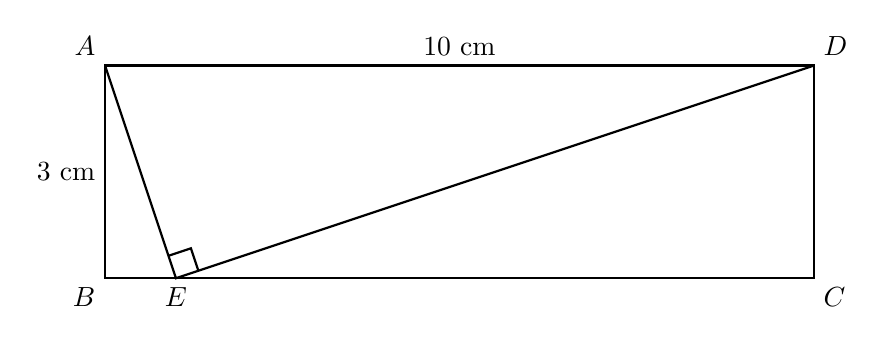
\begin{tikzpicture}[x=0.9cm,y=0.9cm]
\def\rectwidth{10}
\def\rectheight{3}
\def\BE{1}

\coordinate (B) at (0,0);
\coordinate (A) at (0,\rectheight);
\coordinate (C) at (\rectwidth,0);
\coordinate (D) at (\rectwidth,\rectheight);
\coordinate (E) at (\BE,0);

\draw[thick, black] (A) -- (B) -- (C) -- (D) -- cycle;
\draw[thick, black] (A) -- (E) -- (D);

\pic[draw, thick, angle radius=3mm] {right angle=D--E--A};

\node[above left] at (A) {$A$};
\node[below left] at (B) {$B$};
\node[below right] at (C) {$C$};
\node[above right] at (D) {$D$};
\node[below] at (E) {$E$};

\path (A) -- (B) node[midway, left] {$3\text{ cm}$};
\path (A) -- (D) node[midway, above] {$10\text{ cm}$};
\end{tikzpicture}
% end q000659 diagram
\end{center}

\par\vspace*{12pt}
\begin{tabularx}{\linewidth}{@{}>{\bfseries}l Y@{}}
A &
% begin q000659 choice A
$9\text{ cm}^2$
% end q000659 choice A
\\[0.8em]
B &
% begin q000659 choice B
$18\text{ cm}^2$
% end q000659 choice B
\\[0.8em]
C &
% begin q000659 choice C
$41\text{ cm}^2$
% end q000659 choice C
\\[0.8em]
D &
% begin q000659 choice D
$50\text{ cm}^2$
% end q000659 choice D
\\[0.8em]
E &
% begin q000659 choice E
$82\text{ cm}^2$
% end q000659 choice E
\\
\end{tabularx}
\end{enumerate}
\clearpage
\thispagestyle{djspaper}
\vspace*{8pt}
\djsTopicLine{Exponentials \& Logarithms}
\begin{enumerate}[label=\textbf{\arabic*.},leftmargin=*,itemsep=0pt,start=3]
\questionitem[Exponentials \& Logarithms]
% begin q000731 stem
For $1<x<81$, the equation
\[\log_2(\log_3 x)+\log_2\!\left(\log_3\frac{81}{x}\right)=1\]

has two solutions. What is the smaller solution?
% end q000731 stem

\par\vspace*{12pt}
\begin{tabularx}{\linewidth}{@{}>{\bfseries}l Y@{}}
A &
% begin q000731 choice A
$3^{2-\sqrt{3}}$
% end q000731 choice A
\\[0.8em]
B &
% begin q000731 choice B
$3^{2-\sqrt{2}}$
% end q000731 choice B
\\[0.8em]
C &
% begin q000731 choice C
$3^{\sqrt{2}}$
% end q000731 choice C
\\[0.8em]
D &
% begin q000731 choice D
$3^{4-\sqrt{2}}$
% end q000731 choice D
\\[0.8em]
E &
% begin q000731 choice E
$3^{2+\sqrt{2}}$
% end q000731 choice E
\\
\end{tabularx}
\end{enumerate}
\clearpage
\thispagestyle{djspaper}
\vspace*{8pt}
\djsTopicLine{Trigonometry}
\begin{enumerate}[label=\textbf{\arabic*.},leftmargin=*,itemsep=0pt,start=4]
\questionitem[Trigonometry]
% begin q000750 stem
Triangle $ABC$ is right-angled at $A$, and angle $ABC$ is $30^\circ$

The point $D$ is the midpoint of $AB$

If angle $ACD$ is $\theta$, what is $\cos\theta$?
% end q000750 stem

\begin{center}
% begin q000750 diagram
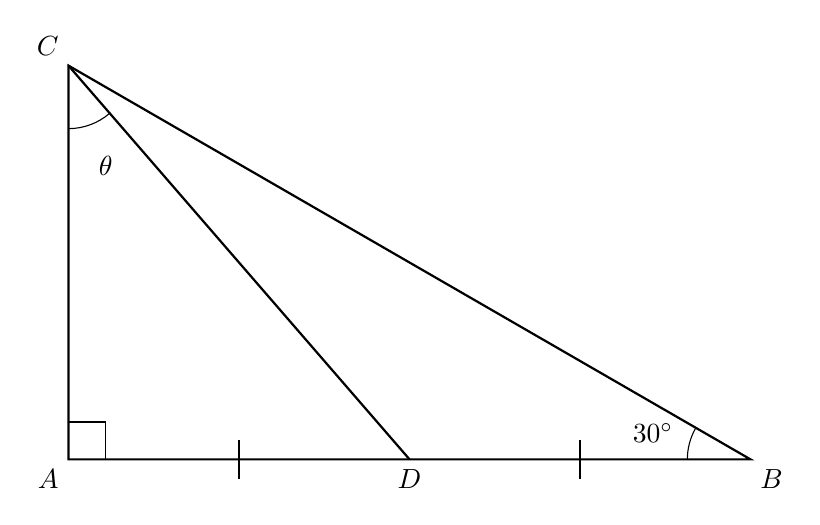
\begin{tikzpicture}[scale=2.5]
\def\height{2}
\pgfmathsetmacro{\base}{sqrt(3)*\height}
\coordinate (A) at (0,0);
\coordinate (B) at (\base,0);
\coordinate (C) at (0,\height);
\coordinate (D) at ($(A)!0.5!(B)$);
\coordinate (TAD) at ($(A)!0.5!(D)$);
\coordinate (TDB) at ($(D)!0.5!(B)$);

\draw[thick,black] (A) -- (B) -- (C) -- cycle;
\draw[thick,black] (C) -- (D);
\draw (A) ++(0.19,0) -- ++(0,0.19) -- ++(-0.19,0);
\foreach \P in {TAD,TDB}{
  \draw[thick] ($ (\P)+(0,-0.10) $) -- ($ (\P)+(0,0.10) $);
}
\pic["$30^\circ$",draw,angle radius=8mm,angle eccentricity=1.6]{angle=C--B--A};
\pic["$\theta$",draw,angle radius=8mm,angle eccentricity=1.7]{angle=A--C--D};

\node[below left] at (A) {$A$};
\node[below right] at (B) {$B$};
\node[above left] at (C) {$C$};
\node[below] at (D) {$D$};
\end{tikzpicture}
% end q000750 diagram
\end{center}

\par\vspace*{12pt}
\begin{tabularx}{\linewidth}{@{}>{\bfseries}l Y@{}}
A &
% begin q000750 choice A
$\dfrac{1}{\sqrt7}$
% end q000750 choice A
\\[0.8em]
B &
% begin q000750 choice B
$\dfrac12$
% end q000750 choice B
\\[0.8em]
C &
% begin q000750 choice C
$\dfrac{\sqrt3}{\sqrt7}$
% end q000750 choice C
\\[0.8em]
D &
% begin q000750 choice D
$\dfrac{2}{\sqrt7}$
% end q000750 choice D
\\[0.8em]
E &
% begin q000750 choice E
$\dfrac{\sqrt3}{2}$
% end q000750 choice E
\\
\end{tabularx}
\end{enumerate}
\clearpage
\thispagestyle{djspaper}
\vspace*{8pt}
\djsTopicLine{Sequences \& Series}
\begin{enumerate}[label=\textbf{\arabic*.},leftmargin=*,itemsep=0pt,start=5]
\questionitem[Sequences \& Series]
% begin q000761 stem
An infinite geometric series has positive first term $a$ and common ratio $r$, where $|r| < 1$.
The sum to infinity of this series is $S$.

A second series is formed by taking every third term of the first series, beginning with the first term:
\[ T = u_1 + u_4 + u_7 + u_{10} + \dots \]
where $u_n$ denotes the $n$th term of the first series.\vspace*{3pt}

What is the maximum possible value of $\dfrac{T}{S}$?
% end q000761 stem

\par\vspace*{12pt}
\begin{tabularx}{\linewidth}{@{}>{\bfseries}l Y@{}}
A &
% begin q000761 choice A
$\dfrac{3}{4}$
% end q000761 choice A
\\[0.8em]
B &
% begin q000761 choice B
$1$
% end q000761 choice B
\\[0.8em]
C &
% begin q000761 choice C
$\dfrac{7}{6}$
% end q000761 choice C
\\[0.8em]
D &
% begin q000761 choice D
$\dfrac{4}{3}$
% end q000761 choice D
\\[0.8em]
E &
% begin q000761 choice E
$\dfrac{3}{2}$
% end q000761 choice E
\\[0.8em]
F &
% begin q000761 choice F
$3$
% end q000761 choice F
\\
\end{tabularx}
\end{enumerate}
\clearpage
\thispagestyle{djspaper}
\vspace*{8pt}
\djsTopicLine{Exponentials \& Logarithms}
\begin{enumerate}[label=\textbf{\arabic*.},leftmargin=*,itemsep=0pt,start=6]
\questionitem[Exponentials \& Logarithms]
% begin q000733 stem
Consider the equation
\[
x^{\log_2(x^2)} - 18 x^{\log_2 x} + 32 = 0
\]

What is the sum of all real solutions to this equation?
% end q000733 stem

\par\vspace*{12pt}
\begin{tabularx}{\linewidth}{@{}>{\bfseries}l Y@{}}
A &
% begin q000733 choice A
$1$
% end q000733 choice A
\\[0.8em]
B &
% begin q000733 choice B
$\dfrac{9}{2}$
% end q000733 choice B
\\[0.8em]
C &
% begin q000733 choice C
$6$
% end q000733 choice C
\\[0.8em]
D &
% begin q000733 choice D
$\dfrac{25}{4}$
% end q000733 choice D
\\[0.8em]
E &
% begin q000733 choice E
$\dfrac{13}{2}$
% end q000733 choice E
\\[0.8em]
F &
% begin q000733 choice F
$\dfrac{27}{4}$
% end q000733 choice F
\\[0.8em]
G &
% begin q000733 choice G
$\dfrac{31}{4}$
% end q000733 choice G
\\[0.8em]
H &
% begin q000733 choice H
$18$
% end q000733 choice H
\\
\end{tabularx}
\end{enumerate}
\clearpage
\thispagestyle{djspaper}
\vspace*{8pt}
\djsTopicLine{Differentiation}
\begin{enumerate}[label=\textbf{\arabic*.},leftmargin=*,itemsep=0pt,start=7]
\questionitem[Differentiation]
% begin q000774 stem
A straight line is tangent to both the curve $y=x^2$ and the curve $y=\dfrac{1}{x}$, where $x\ne0$

At what value of $x$ does this line cross the $x$-axis?
% end q000774 stem

\par\vspace*{12pt}
\begin{tabularx}{\linewidth}{@{}>{\bfseries}l Y@{}}
A &
% begin q000774 choice A
$-2$
% end q000774 choice A
\\[0.8em]
B &
% begin q000774 choice B
$-\dfrac{3}{2}$
% end q000774 choice B
\\[0.8em]
C &
% begin q000774 choice C
$-1$
% end q000774 choice C
\\[0.8em]
D &
% begin q000774 choice D
$-\dfrac{1}{2}$
% end q000774 choice D
\\[0.8em]
E &
% begin q000774 choice E
$-\dfrac{1}{4}$
% end q000774 choice E
\\
\end{tabularx}
\end{enumerate}
\clearpage
\thispagestyle{djspaper}
\vspace*{8pt}
\djsTopicLine{Sequences \& Series}
\begin{enumerate}[label=\textbf{\arabic*.},leftmargin=*,itemsep=0pt,start=8]
\questionitem[Sequences \& Series]
% begin q000778 stem
Five positive numbers are consecutive terms of a geometric sequence 

The middle three have sum $14$ and multiply to make $8$

What is the sum of all five numbers?
% end q000778 stem

\par\vspace*{12pt}
\begin{tabularx}{\linewidth}{@{}>{\bfseries}l Y@{}}
A &
% begin q000778 choice A
$74$
% end q000778 choice A
\\[0.8em]
B &
% begin q000778 choice B
$78$
% end q000778 choice B
\\[0.8em]
C &
% begin q000778 choice C
$80$
% end q000778 choice C
\\[0.8em]
D &
% begin q000778 choice D
$82$
% end q000778 choice D
\\[0.8em]
E &
% begin q000778 choice E
$84$
% end q000778 choice E
\\[0.8em]
F &
% begin q000778 choice F
$86$
% end q000778 choice F
\\
\end{tabularx}
\end{enumerate}
\clearpage
\thispagestyle{djspaper}
\vspace*{8pt}
\djsTopicLine{Probability \& Counting}
\begin{enumerate}[label=\textbf{\arabic*.},leftmargin=*,itemsep=0pt,start=9]
\questionitem[Probability \& Counting]
% begin q000767 stem
A bag contains $3$ red balls and $2$ blue balls. 

Two balls are drawn without replacement. 

If they are the same colour, both are returned to the bag. If they are different colours, both are left out.

A ball is then drawn from the bag.

What is the probability that this final ball is red?
% end q000767 stem

\par\vspace*{12pt}
\begin{tabularx}{\linewidth}{@{}>{\bfseries}l Y@{}}
A &
% begin q000767 choice A
$\dfrac{3}{5}$
% end q000767 choice A
\\[0.8em]
B &
% begin q000767 choice B
$\dfrac{19}{30}$
% end q000767 choice B
\\[0.8em]
C &
% begin q000767 choice C
$\dfrac{16}{25}$
% end q000767 choice C
\\[0.8em]
D &
% begin q000767 choice D
$\dfrac{2}{3}$
% end q000767 choice D
\\[0.8em]
E &
% begin q000767 choice E
$\dfrac{7}{10}$
% end q000767 choice E
\\
\end{tabularx}
\end{enumerate}
\clearpage
\thispagestyle{djspaper}
\vspace*{8pt}
\djsTopicLine{Algebra}
\begin{enumerate}[label=\textbf{\arabic*.},leftmargin=*,itemsep=0pt,start=10]
\questionitem[Algebra]
% begin q000779 stem
Real numbers $x$ and $y$ satisfy
\[x+y=xy\]
and
\[(x-1)^2+(y-1)^2=7\]

What are the possible values of $xy$?
% end q000779 stem

\par\vspace*{12pt}
\begin{tabularx}{\linewidth}{@{}>{\bfseries}l Y@{}}
A &
% begin q000779 choice A
$-5$ and $1$
% end q000779 choice A
\\[0.8em]
B &
% begin q000779 choice B
$-3$ and $3$
% end q000779 choice B
\\[0.8em]
C &
% begin q000779 choice C
$-1$ and $3$
% end q000779 choice C
\\[0.8em]
D &
% begin q000779 choice D
$-1$ and $5$
% end q000779 choice D
\\[0.8em]
E &
% begin q000779 choice E
$1$ and $5$
% end q000779 choice E
\\
\end{tabularx}
\end{enumerate}
\clearpage
\thispagestyle{djspaper}
\vspace*{8pt}
\djsTopicLine{Probability \& Counting}
\begin{enumerate}[label=\textbf{\arabic*.},leftmargin=*,itemsep=0pt,start=11]
\questionitem[Probability \& Counting]
% begin q000041 stem
Find the coefficient of $x^3y^2$ in the expansion of \[(1-2x+y)^8\]
% end q000041 stem

\par\vspace*{12pt}
\begin{tabularx}{\linewidth}{@{}>{\bfseries}l Y@{}}
A &
% begin q000041 choice A
$-17920$
% end q000041 choice A
\\[0.8em]
B &
% begin q000041 choice B
$-13440$
% end q000041 choice B
\\[0.8em]
C &
% begin q000041 choice C
$-4480$
% end q000041 choice C
\\[0.8em]
D &
% begin q000041 choice D
$-560$
% end q000041 choice D
\\[0.8em]
E &
% begin q000041 choice E
$560$
% end q000041 choice E
\\[0.8em]
F &
% begin q000041 choice F
$4480$
% end q000041 choice F
\\[0.8em]
G &
% begin q000041 choice G
$17920$
% end q000041 choice G
\\
\end{tabularx}
\end{enumerate}
\clearpage
\thispagestyle{djspaper}
\vspace*{8pt}
\djsTopicLine{Inequalities}
\begin{enumerate}[label=\textbf{\arabic*.},leftmargin=*,itemsep=0pt,start=12]
\questionitem[Inequalities]
% begin q000773 stem
The function $f$ is defined for all real $x$ by
\[
f(x)=\frac{x^{2}+4x+1}{x^{2}+1}
\]

Which of the following gives all possible values of \(f(x)\) as \(x\) varies over the real numbers?
% end q000773 stem

\par\vspace*{12pt}
\begin{tabularx}{\linewidth}{@{}>{\bfseries}l Y@{}}
A &
% begin q000773 choice A
$-1 \le f(x) \le 3$
% end q000773 choice A
\\[0.8em]
B &
% begin q000773 choice B
$f(x) \le -1$ or $f(x) \ge 3$
% end q000773 choice B
\\[0.8em]
C &
% begin q000773 choice C
$1 \le f(x) \le 3$
% end q000773 choice C
\\[0.8em]
D &
% begin q000773 choice D
$-3 \le f(x) \le 1$
% end q000773 choice D
\\[0.8em]
E &
% begin q000773 choice E
$-1 \le f(x) \le 1$
% end q000773 choice E
\\[0.8em]
F &
% begin q000773 choice F
$f(x)$ can take all real values
% end q000773 choice F
\\
\end{tabularx}
\end{enumerate}
\clearpage
\thispagestyle{djspaper}
\vspace*{8pt}
\djsTopicLine{Coordinate Geometry}
\begin{enumerate}[label=\textbf{\arabic*.},leftmargin=*,itemsep=0pt,start=13]
\questionitem[Coordinate Geometry]
% begin q000620 stem
The points $P$ and $R$ lie on the curve $y=x^2$ and have $x$-coordinates $1$ and $3$, respectively. The tangents to the curve at $P$ and $R$ meet at $Q$.

The area enclosed by the curve and the line segment $PR$ is $A$. The area of triangle $PQR$ is $B$.

What is the value of $\dfrac{A}{B}$?
% end q000620 stem

\begin{center}
% begin q000620 diagram
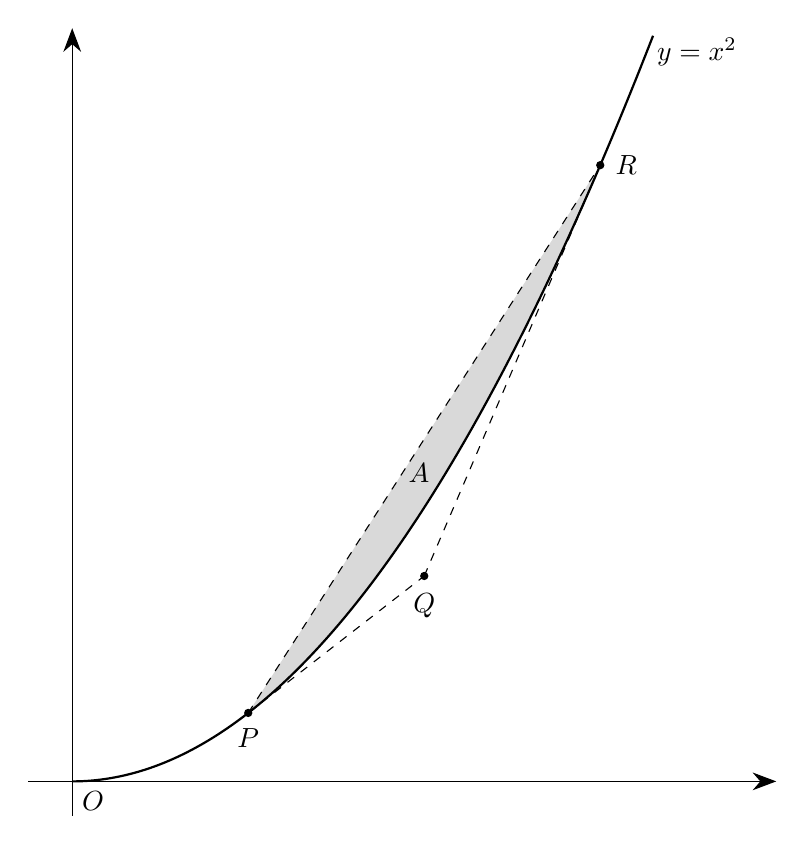
\begin{tikzpicture}
\begin{axis}[
    width=9.5cm,
    height=10cm,
    scale only axis,
    axis lines=middle,
    axis line style={solid, black, -{Stealth[length=3mm]}},
    axis on top,
    xmin=-0.25, xmax=4,
    ymin=-0.5, ymax=11,
    xtick=\empty,
    ytick=\empty,
    clip=true,
    clip mode=individual
]
% Exact paths defining the shaded region
\addplot[draw=none, name path=chord, domain=1:3, samples=2] {4*x-3};
\addplot[draw=none, name path=parabolaRegion, domain=1:3, samples=100] {x^2};
\addplot[gray!30] fill between[of=chord and parabolaRegion];

% Parabola and triangle boundary
\addplot[thick, black, domain=0:3.3, samples=150] {x^2}
    node[pos=0.98, right] {$y=x^2$};
\addplot[dashed, black, domain=1:3, samples=2] {4*x-3};
\addplot[dashed, black, domain=1:2, samples=2] {2*x-1};
\addplot[dashed, black, domain=2:3, samples=2] {6*x-9};

% Marked points
\fill (axis cs:1,1) circle (1.5pt);
\fill (axis cs:2,3) circle (1.5pt);
\fill (axis cs:3,9) circle (1.5pt);
\node[right=2pt, below=2pt] at (axis cs:1,1) {$P$};
\node[below=3pt] at (axis cs:2,3) {$Q$};
\node[right=2pt] at (axis cs:3,9) {$R$};

% Region and origin labels
\node at (axis cs:1.97,4.5) {$A$};
\node[below right] at (axis cs:0,0) {$O$};
\end{axis}
\end{tikzpicture}
% end q000620 diagram
\end{center}

\par\vspace*{12pt}
\begin{tabularx}{\linewidth}{@{}>{\bfseries}l Y@{}}
A &
% begin q000620 choice A
$\dfrac{1}{3}$
% end q000620 choice A
\\[0.8em]
B &
% begin q000620 choice B
$\dfrac{1}{2}$
% end q000620 choice B
\\[0.8em]
C &
% begin q000620 choice C
$\dfrac{2}{3}$
% end q000620 choice C
\\[0.8em]
D &
% begin q000620 choice D
$\dfrac{3}{4}$
% end q000620 choice D
\\[0.8em]
E &
% begin q000620 choice E
$\dfrac{3}{2}$
% end q000620 choice E
\\
\end{tabularx}
\end{enumerate}
\clearpage
\thispagestyle{djspaper}
\vspace*{8pt}
\djsTopicLine{Integration}
\begin{enumerate}[label=\textbf{\arabic*.},leftmargin=*,itemsep=0pt,start=14]
\questionitem[Integration]
% begin q000627 stem
The diagram shows the graph of $y=f(x)$ for $0\le x\le 8$. The graph is made up of straight line segments joining the points $(0,2)$, $(2,2)$, $(5,-4)$, $(6,0)$ and $(8,1)$.

The function $g$ is defined by
\[g(x)=\int_0^x f(t)\,\mathrm{d}t \qquad \text{for } 0\le x\le 8\]

How many values of $x$ with $0\le x\le 8$ satisfy $g(x)=0$?
% end q000627 stem

\begin{center}
% begin q000627 diagram
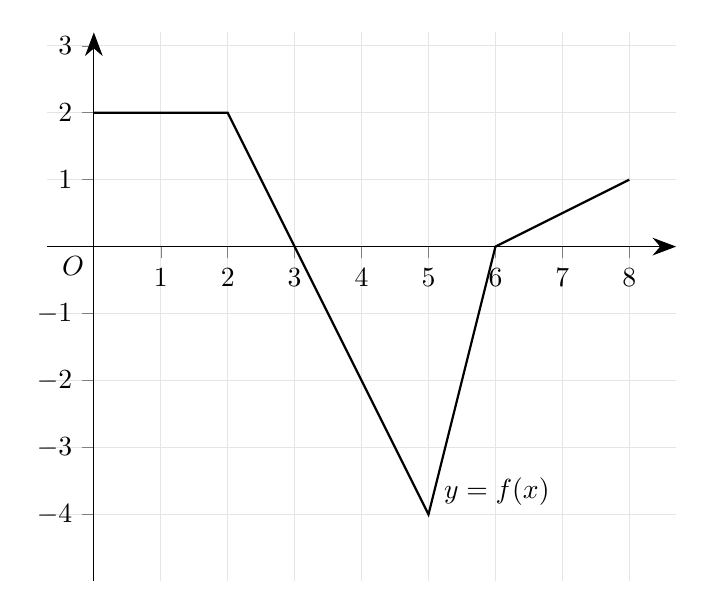
\begin{tikzpicture}
\begin{axis}[
    x=0.85cm,
    y=0.85cm,
    scale only axis,
    axis lines=middle,
    axis line style={-{Stealth[length=3mm]}, black},
    xmin=-0.7, xmax=8.7,
    ymin=-5, ymax=3.2,
    xtick={0,1,2,3,4,5,6,7,8},
    xticklabels={,$1$,$2$,$3$,$4$,$5$,$6$,$7$,$8$},
    ytick={-4,-3,-2,-1,0,1,2,3},
    yticklabels={$-4$,$-3$,$-2$,$-1$,,$1$,$2$,$3$},
    tick align=outside,
    grid=major,
    grid style={gray!20, thin},
    clip=true
]

\addplot[
    thick,
    black,
    mark=none
] coordinates {
    (0,2) (2,2) (5,-4) (6,0) (8,1)
} node[pos=0.6, below right, yshift=9pt] {$y=f(x)$};

\node[below left] at (axis cs:0,0) {$O$};
\node[right] at (axis cs:8.7,0) {$x$};
\node[above] at (axis cs:0,3.2) {$y$};

\end{axis}
\end{tikzpicture}
% end q000627 diagram
\end{center}

\par\vspace*{12pt}
\begin{tabularx}{\linewidth}{@{}>{\bfseries}l Y@{}}
A &
% begin q000627 choice A
$0$
% end q000627 choice A
\\[0.8em]
B &
% begin q000627 choice B
$1$
% end q000627 choice B
\\[0.8em]
C &
% begin q000627 choice C
$2$
% end q000627 choice C
\\[0.8em]
D &
% begin q000627 choice D
$3$
% end q000627 choice D
\\[0.8em]
E &
% begin q000627 choice E
$4$
% end q000627 choice E
\\[0.8em]
F &
% begin q000627 choice F
$5$
% end q000627 choice F
\\
\end{tabularx}
\end{enumerate}
\clearpage
\thispagestyle{djspaper}
\vspace*{8pt}
\djsTopicLine{Number}
\begin{enumerate}[label=\textbf{\arabic*.},leftmargin=*,itemsep=0pt,start=15]
\questionitem[Number]
% begin q000725 stem
Let $k$ be a positive integer, and let $N=2^4\times3^k$

The product of all the positive factors of $N$ is the fourth power of an integer. 

What is the smallest possible value of $k$?
% end q000725 stem

\par\vspace*{12pt}
\begin{tabularx}{\linewidth}{@{}>{\bfseries}l Y@{}}
A &
% begin q000725 choice A
$1$
% end q000725 choice A
\\[0.8em]
B &
% begin q000725 choice B
$2$
% end q000725 choice B
\\[0.8em]
C &
% begin q000725 choice C
$3$
% end q000725 choice C
\\[0.8em]
D &
% begin q000725 choice D
$5$
% end q000725 choice D
\\[0.8em]
E &
% begin q000725 choice E
$7$
% end q000725 choice E
\\[0.8em]
F &
% begin q000725 choice F
$8$
% end q000725 choice F
\\
\end{tabularx}
\end{enumerate}
\clearpage
\thispagestyle{djspaper}
\vspace*{8pt}
\djsTopicLine{Polynomials}
\begin{enumerate}[label=\textbf{\arabic*.},leftmargin=*,itemsep=0pt,start=16]
\questionitem[Polynomials]
% begin q000777 stem
A quadratic polynomial $f$ has roots $1$ and $3$.

The equation $f(f(x))=0$ has exactly three distinct real solutions. 

What is the value of $f(0)$?
% end q000777 stem

\par\vspace*{12pt}
\begin{tabularx}{\linewidth}{@{}>{\bfseries}l Y@{}}
A &
% begin q000777 choice A
$-9$
% end q000777 choice A
\\[0.8em]
B &
% begin q000777 choice B
$-3$
% end q000777 choice B
\\[0.8em]
C &
% begin q000777 choice C
$-1$
% end q000777 choice C
\\[0.8em]
D &
% begin q000777 choice D
$3$
% end q000777 choice D
\\[0.8em]
E &
% begin q000777 choice E
$9$
% end q000777 choice E
\\
\end{tabularx}
\end{enumerate}
\clearpage
\thispagestyle{djspaper}
\vspace*{8pt}
\djsTopicLine{Trigonometry}
\begin{enumerate}[label=\textbf{\arabic*.},leftmargin=*,itemsep=0pt,start=17]
\questionitem[Trigonometry]
% begin q000719 stem
A triangle has an angle of $120^\circ$ 

The perimeter of the triangle is $15$, and its area is $\dfrac{15\sqrt{3}}{4}$ \vspace*{5pt}

What is the length of the longest side of the triangle?
% end q000719 stem

\par\vspace*{12pt}
\begin{tabularx}{\linewidth}{@{}>{\bfseries}l Y@{}}
A &
% begin q000719 choice A
$5$
% end q000719 choice A
\\[0.8em]
B &
% begin q000719 choice B
$\dfrac{11}{2}$
% end q000719 choice B
\\[0.8em]
C &
% begin q000719 choice C
$6$
% end q000719 choice C
\\[0.8em]
D &
% begin q000719 choice D
$\dfrac{13}{2}$
% end q000719 choice D
\\[0.8em]
E &
% begin q000719 choice E
$7$
% end q000719 choice E
\\[0.8em]
F &
% begin q000719 choice F
$\dfrac{15}{2}$
% end q000719 choice F
\\[0.8em]
G &
% begin q000719 choice G
$8$
% end q000719 choice G
\\
\end{tabularx}
\end{enumerate}
\clearpage
\thispagestyle{djspaper}
\vspace*{8pt}
\djsTopicLine{Coordinate Geometry}
\begin{enumerate}[label=\textbf{\arabic*.},leftmargin=*,itemsep=0pt,start=18]
\questionitem[Coordinate Geometry]
% begin q000653 stem
The point $A$ has coordinates $(-7,-5)$ and the point $B$ has coordinates $(23,45)$.

How many points on the straight line segment $AB$ have both coordinates equal to integers, not counting $A$ and $B$ themselves?
% end q000653 stem

\par\vspace*{12pt}
\begin{tabularx}{\linewidth}{@{}>{\bfseries}l Y@{}}
A &
% begin q000653 choice A
$4$
% end q000653 choice A
\\[0.8em]
B &
% begin q000653 choice B
$5$
% end q000653 choice B
\\[0.8em]
C &
% begin q000653 choice C
$9$
% end q000653 choice C
\\[0.8em]
D &
% begin q000653 choice D
$10$
% end q000653 choice D
\\[0.8em]
E &
% begin q000653 choice E
$11$
% end q000653 choice E
\\[0.8em]
F &
% begin q000653 choice F
$29$
% end q000653 choice F
\\[0.8em]
G &
% begin q000653 choice G
$49$
% end q000653 choice G
\\
\end{tabularx}
\end{enumerate}
\clearpage
\thispagestyle{djspaper}
\vspace*{8pt}
\djsTopicLine{Algebra}
\begin{enumerate}[label=\textbf{\arabic*.},leftmargin=*,itemsep=0pt,start=19]
\questionitem[Algebra]
% begin q000751 stem
The positive real numbers $x$ and $y$ satisfy the equations
\[x\sqrt{y} + y\sqrt{x} = 8\]
and
\[x\sqrt{x} + y\sqrt{y} = 40\]
What is the value of $x + y$?
% end q000751 stem

\par\vspace*{12pt}
\begin{tabularx}{\linewidth}{@{}>{\bfseries}l Y@{}}
A &
% begin q000751 choice A
$6$
% end q000751 choice A
\\[0.8em]
B &
% begin q000751 choice B
$8$
% end q000751 choice B
\\[0.8em]
C &
% begin q000751 choice C
$10$
% end q000751 choice C
\\[0.8em]
D &
% begin q000751 choice D
$12$
% end q000751 choice D
\\[0.8em]
E &
% begin q000751 choice E
$14$
% end q000751 choice E
\\[0.8em]
F &
% begin q000751 choice F
$16$
% end q000751 choice F
\\
\end{tabularx}
\end{enumerate}
\clearpage
\thispagestyle{djspaper}
\vspace*{8pt}
\djsTopicLine{Integration}
\begin{enumerate}[label=\textbf{\arabic*.},leftmargin=*,itemsep=0pt,start=20]
\questionitem[Integration]
% begin q000729 stem
Let $f$ be a polynomial of degree at most $3$ with real coefficients.

For $t>0$, define
\[
D(t)=\int_0^t f(x)\,\mathrm{d}x-\int_{-t}^0 f(x)\,\mathrm{d}x
\]
Which of the following statements are true?
\[
\begin{array}{@{}ll@{}}
\textbf{I} & \text{If }f(x)=f(-x)\text{ for every real }x,\text{ then }D(1)=0 \\[5pt]
\textbf{II} & \text{If }D(1)=0,\text{ then }f(x)=f(-x)\text{ for every real }x \\[5pt]
\textbf{III} & \text{If }D(1)=D(2)=0,\text{ then }f(x)=f(-x)\text{ for every real }x \\[5pt]
\end{array}
\]
% end q000729 stem

\par\vspace*{12pt}
\begin{tabularx}{\linewidth}{@{}>{\bfseries}l Y@{}}
A &
% begin q000729 choice A
None of them
% end q000729 choice A
\\[0.8em]
B &
% begin q000729 choice B
I only
% end q000729 choice B
\\[0.8em]
C &
% begin q000729 choice C
II only
% end q000729 choice C
\\[0.8em]
D &
% begin q000729 choice D
III only
% end q000729 choice D
\\[0.8em]
E &
% begin q000729 choice E
I and II only
% end q000729 choice E
\\[0.8em]
F &
% begin q000729 choice F
I and III only
% end q000729 choice F
\\[0.8em]
G &
% begin q000729 choice G
II and III only
% end q000729 choice G
\\[0.8em]
H &
% begin q000729 choice H
I, II and III
% end q000729 choice H
\\
\end{tabularx}
\end{enumerate}
\end{document}
